\chapter{Methodology}\label{sec:chapter3}

The framework established in the previous chapters has prioritized the need for cavities with high-quality factors in magnetic fields for axion detector experiments. This chapter describes:

\begin{itemize}
    \item Fabrication methods to make Nb$_3$Sn films 
    \item Methods to analyze the structure and composition of Nb$_3$Sn film samples 
    \item Methods to characterize the normal-state and superconducting properties of Nb$_3$Sn film samples
    \item Methods to characterize the RF properties of conductors and superconductors
\end{itemize}

After fabrication, the film quality of small samples can be characterized using critical temperature ($T_c$) measurements, visible light microscopy, and scanning electron microscopy (SEM) with energy-dispersive spectroscopy (EDS). These techniques require little setup time and provide a wealth of information about the films.  It should be noted that building an entire cavity is often necessary to assess the RF behavior of a film or material, which will be covered in later chapters, because this is the end product of this dissertation.



%\begin{itemize}
%    \item Small sample screening ($T_c$, SEM/EDS) to optimize fabrication
%    \item RF cavity testing ($Q$ vs $T$, $Q$ vs $B$) to validate performance under detector conditions
%\end{itemize}




\section{Making \texorpdfstring{Nb$_3$Sn}{Nb3Sn} Thin Films}

Standard fabrication techniques are described in the following thin-film textbook~\cite{seshanHandbookThinFilm2002}. The specific recipes used in this work to fabricate Nb$_3$Sn are provided in Sec.~\ref{sec:nb3snresults}.


    \subsection{Substrate Preparation}
    
    Surface preparation is critical for thin film adhesion and quality. Substrates underwent mechanical polishing from carbide paper through diamond slurry to colloidal silica, progressively reducing surface roughness to $<50$~nm RMS (detailed protocol in Appendix~\ref{appsec:substrateprep}). Substrates were cut differently depending on the use case: $<1$~cm square (small samples), 2-inch disk (mushroom cavity), and custom geometries (RF measurements).

    \subsection{Thermal Evaporation}
    
    Thermal evaporation is a physical vapor deposition technique where source material is heated to high temperatures in vacuum until it vaporizes and condenses on a substrate (Fig.~\ref{fig:ThermalEvap}). Evaporation occurs when atoms gain sufficient thermal energy to overcome surface binding forces. An electric current passes through a refractory-metal container (boat, basket, or crucible) containing the source material. The container's electrical resistance causes Joule heating ($P = I^2R$), and as current increases, the temperature rises until the source material reaches its vaporization temperature. A standard heating element is tungsten (melting point 3422~°C), chosen for its high melting point and low reactivity. 

    \begin{figure}[tb]
        \centering
        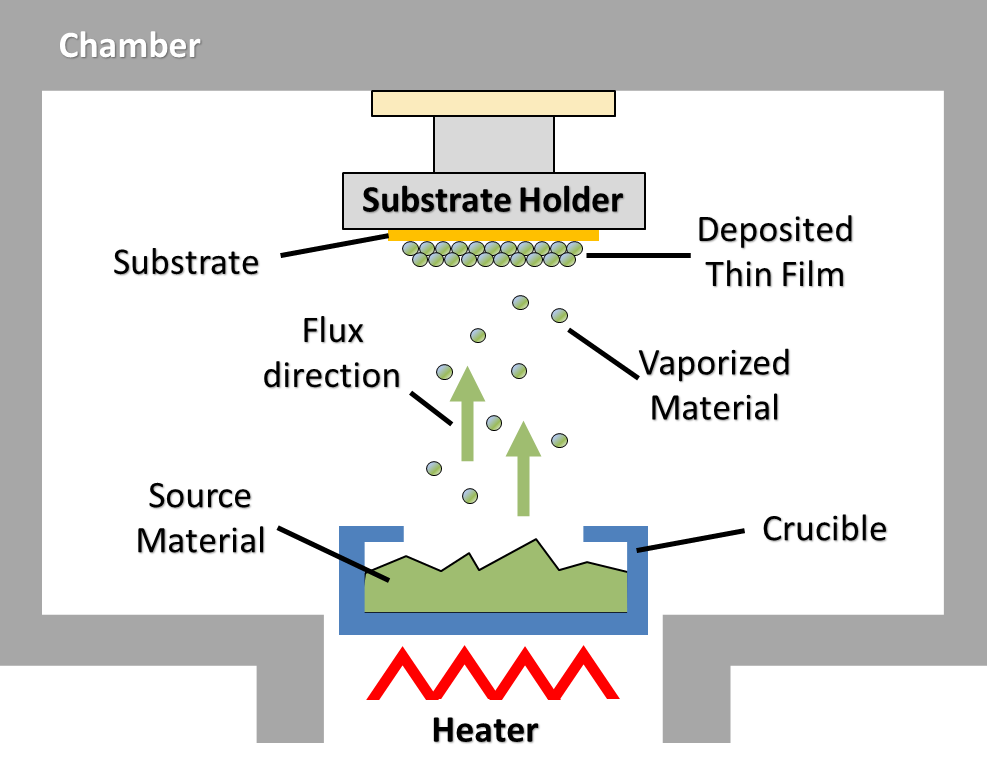
\includegraphics[width=.8\textwidth]{images/Metallurgy/ThermalEvap.png}
        \caption[Source material heated and evaporated onto a target.]{Source material heated and evaporated onto a target. Material is moving from a hot location (crucible) to a cold location (substrate).}
        \label{fig:ThermalEvap}
    \end{figure}

    The atomic-scale deposition process involves several sequential steps. At the source, thermal energy drives atomic diffusion towards the surface, followed by desorption when atoms gain energy exceeding the surface work function. The desorbed atoms undergo ballistic motion through the vacuum chamber (enabled by mean free paths exceeding chamber dimensions at typical pressures), then adsorb onto the substrate surface. Surface dynamics include ad-atom lateral mobility, re-desorption events, atomic displacement by incoming flux (``atomic peening"), and defect formation when mobility is insufficient for ideal crystal growth. Bulk diffusion is generally negligible at typical substrate temperatures.
    
    The vapor pressure of a material varies with temperature (Fig.~\ref{fig:VaporPressure}). For materials relevant to Nb$_3$Sn synthesis: tin has a relatively low melting point of 232~°C and evaporates readily, while copper melts at 1085~°C and niobium at 2477~°C. The chamber pressure must be significantly lower than the material's vapor pressure to allow free-molecular flow. At typical chamber pressures ($\sim10^{-6}$ Torr), the mean free path exceeds the chamber dimensions, enabling line-of-sight deposition.

        
    \begin{figure}[tb]
        \centering
        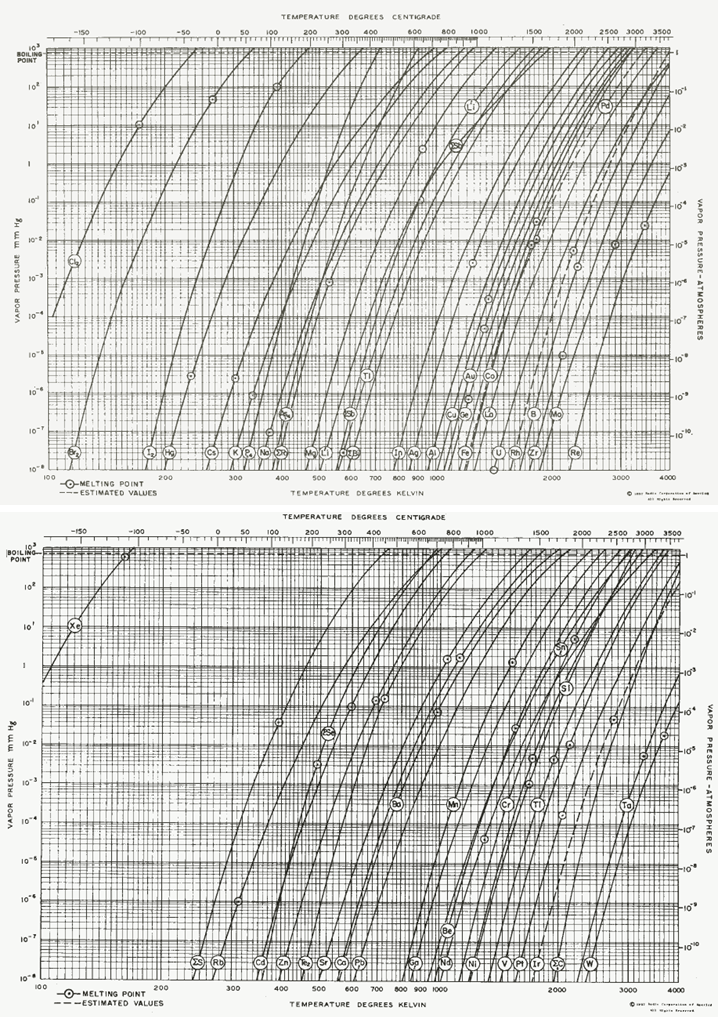
\includegraphics[width=.8\textwidth]{images/Metallurgy/VaporPressure2.png}
        \caption{Vapor pressure curves for common elements \cite{leonmaisselHandbookThinFilm1995}.}
        \label{fig:VaporPressure}
    \end{figure}
    \FloatBarrier
    
    When evaporating alloys or co-evaporating multiple elements, components evaporate at different rates according to their individual vapor pressures, thereby altering the film's elemental composition relative to the source elemental composition. This is particularly important for materials such as Cu-Sn alloys, where tin's higher vapor pressure leads to preferential evaporation. The deposition rate follows a cosine distribution from the source, with maximum thickness directly above the source and decreasing with increasing angle. Thickness monitoring is typically achieved using a quartz crystal microbalance (QCM) or through post-deposition techniques such as profilometry or cross-sectional imaging.
    
    Thermal evaporation offers several advantages, including high-purity depositions, reasonable rate control, and the ability to deposit multiple materials sequentially without breaking vacuum. However, it is limited to line-of-sight deposition, resulting in poor step coverage, non-uniform thicknesses over large areas, and difficulty in depositing very high-melting-point materials~\cite{leonmaisselHandbookThinFilm1995}. Pre-outgassing the source material at a moderate temperature before evaporation helps reduce contamination from adsorbed gases. While substrate heating promotes crystallinity and substrate rotation could improve thickness uniformity, the evaporation chamber was not equipped with these tools, which constrained the work in this dissertation. Small samples were used to mitigate the adverse effects of these constraints. However, in the large RF samples used, defects were found that may have resulted from these constraints. 

    \subsection{Magnetron Sputtering}

    In a weak vacuum, a high electric field can ionize gas and produce a plasma for deposition. The Paschen condition specifies the required field or voltage for plasma discharge~\cite{paschenUeberFunkenubergangLuft1889}. The gas type and pressure are selected based on voltage and chamber characteristics. Inert gas ions are typically used to avoid unwanted reactions with the target material. Ions from the resulting discharge can have high energy, more than sufficient to liberate atoms from the surface of a metal target, which is called sputtering.

    The inert gas plasma (typically Ar) accelerates ions toward a target material, where momentum transfer ejects target atoms. These atoms traverse the vacuum chamber and nucleate on a substrate, building a thin film atom by atom. Control over plasma conditions, chamber pressure, and substrate temperature allows tuning of film composition, microstructure, and deposition rate.

    Magnetic fields increase the efficiency of harvesting gas ions for sputtering. The magnetic field contours trap ions near the target (Fig.~\ref{fig:MagnetronSputtering}), confining the plasma to a dense region above the target and increasing deposition rates by $10-100\times$ while reducing substrate heating~\cite{mattoxHandbookPhysicalVapor2010}. DC sputtering was used for all metal depositions in this work. RF sputtering at 13.56~MHz was used only for in-situ substrate cleaning before deposition.

    \begin{figure}[tb]
        \centering
        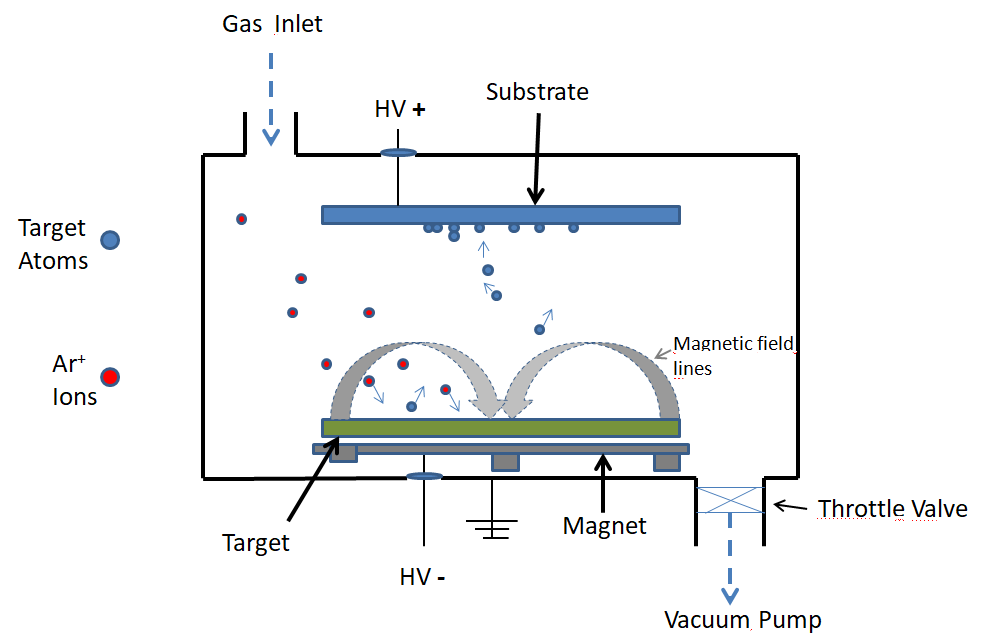
\includegraphics[width=\textwidth]{images/Metallurgy/MagnetronSputtering.png}
        \caption[An ultra-high vacuum chamber with a working gas (Argon) that hits the target material and liberates target atoms.]{An ultra-high vacuum chamber with a working gas (Argon) that hits the target material and liberates target atoms. The argon atoms hit the target many times over as the magnet underneath the target accelerates them back to the target \cite{mullerIntroductionVacuumCoating}.}
        \label{fig:MagnetronSputtering}
    \end{figure}
    \FloatBarrier
        
    Sputtering can deposit any material regardless of melting point, unlike thermal evaporation. Sputtered films are generally denser and more adherent due to the higher kinetic energy of arriving atoms~\cite{mattoxHandbookPhysicalVapor2010}. When sputtered atoms arrive at the substrate surface, they become adatoms with limited mobility. The substrate temperature and kinetic energy of arriving atoms determine how far adatoms can diffuse before they nucleate at favorable sites or join existing islands. The competition between arrival rate and surface diffusion rate determines the resulting film morphology~\cite{ohringMaterialsScienceThin2002}.
    
    This relationship is captured by the Thornton structure zone model (Fig.~\ref{fig:ThorntonDiagram}), which maps film microstructure as a function of homologous temperature $T/T_m$ (substrate temperature normalized to the melting point) and working gas pressure. At low $T/T_m$ and high pressure (Zone 1), adatom mobility is limited, and porous columnar films with voided grain boundaries form. As $T/T_m$ increases or pressure decreases (Zone T and Zone 2), surface diffusion increases and adatoms can fill voids, producing denser columnar grains. At the highest $T/T_m$ (Zone 3), bulk diffusion dominates and large equiaxed grains form.
    
    For Nb deposition at 8~mTorr Ar, a substrate temperature of 200$^\circ$C gives $T/T_m \approx 0.17$ ($T_m = 2477^\circ$C for Nb), placing the film in Zone 1 or the Zone T boundary. Columnar growth with voided boundaries is expected. At 700$^\circ$C, $T/T_m \approx 0.35$, which falls in Zone 2 where surface diffusion produces denser columnar films with fewer voids. The moderate Ar pressure of 8~mTorr allows sputtered atoms to retain kinetic energy upon arrival, promoting adatom mobility compared to higher pressures where gas-phase scattering thermalizes the arriving flux.
    
    \begin{figure}[tb]
        \centering
        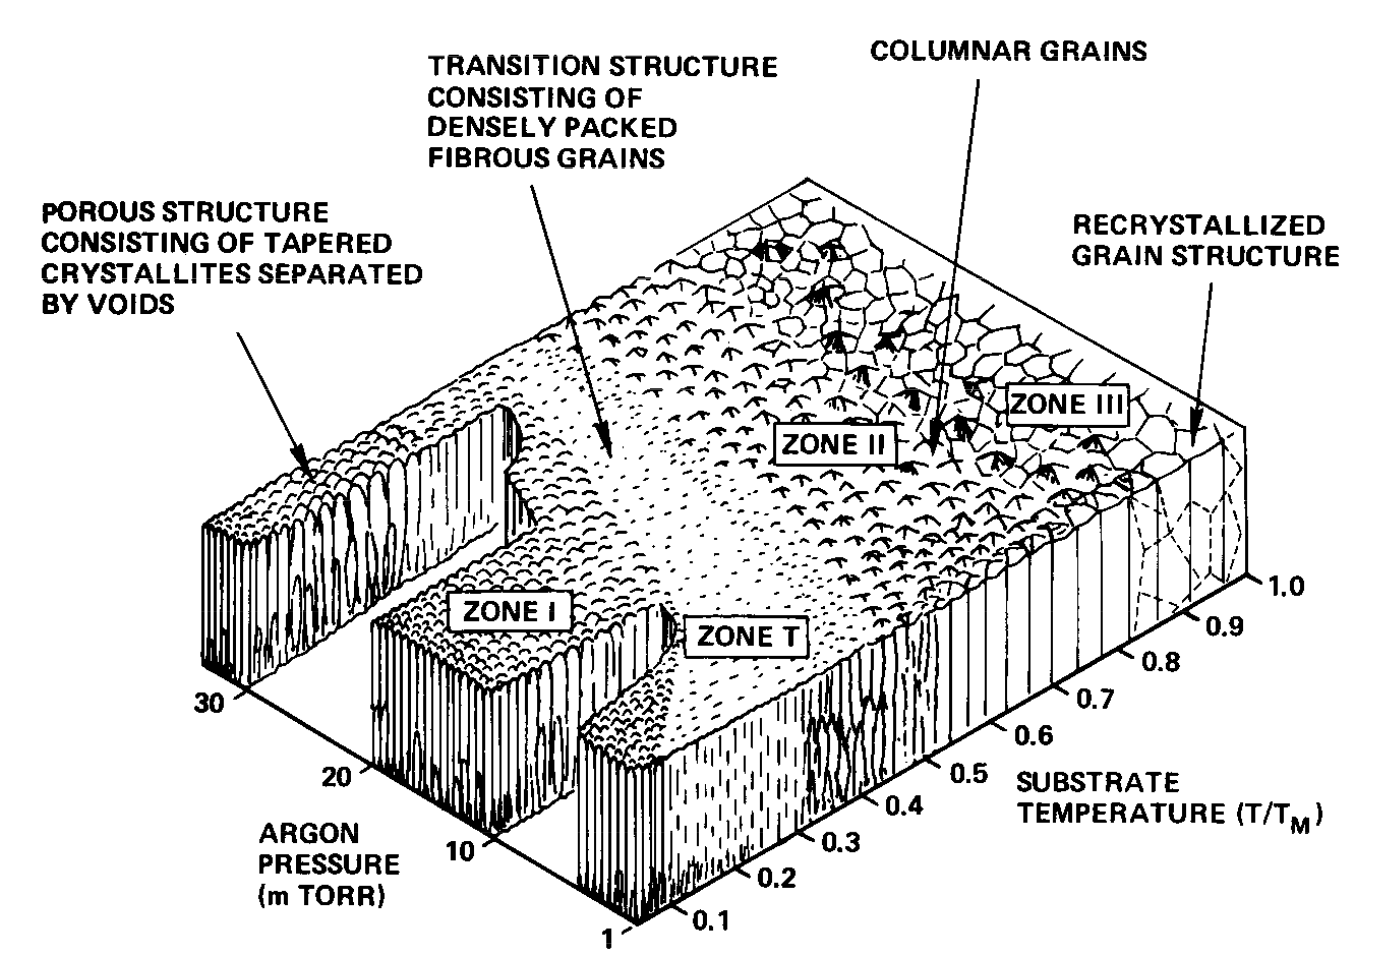
\includegraphics[width=\textwidth]{images/Metallurgy/ThorntonDiagram.png}
        \caption{Thornton structure zone model diagram from~\cite{thorntonInfluenceSubstrateTemperature1975}.}
        \label{fig:ThorntonDiagram}
    \end{figure}
    \FloatBarrier

    \subsection{Post-Deposition Processing}
    
    \subsubsection{Heat-Treatment}
        
    As discussed in more detail later, this dissertation relies upon a diffusion reaction between Cu-Sn and Nb to form Nb$_3$Sn. A necessary step in Nb$_3$Sn film fabrication is a heat treatment in which the film materials are held at high temperatures to enable diffusion reactions. Ultra-high vacuum (UHV) furnaces enable high-temperature reactions in clean environments. Oxygen, nitrogen, and other impurities are problematic in many types of reactions~\cite{Sun:2023ejj}, so UHV furnaces reduce air impurities so the resulting reaction has low impurity content. Ambient pressure is at 1 atm = 760 Torr, high-vacuum pressure is considered $10^{-3}$~to~$10^{-7}$~Torr, and ultra-high vacuum is $10^{-7}$~to~$10^{-12}$~Torr~\cite{rothVacuumTechnology2012}. 
    
    Impurities collect on the surface of newly reacted or deposited material. The rate at which these impurity monolayers form is proportional to the background pressure. The time to form one monolayer of residual gas on a surface is approximately $t_\text{{monolayer}} \approx 3 \times 10^{-8}/P$~seconds, where $P$ is pressure in Torr \cite{ohringMaterialsScienceThin2002}. For example, at atmospheric pressure, a monolayer forms in about three nanoseconds, at $10^{-6}$~Torr in three milliseconds, and at $10^{-9}$~Torr in 3 seconds. This means that even during high-vacuum heat treatments lasting several hours, surfaces are continuously exposed to impurity adsorption. 
    
    Positive-pressure argon furnaces allow further impurity reduction by first pumping down to vacuum, then adding a non-reactive gas until a positive pressure is reached. Continual argon flows through the chamber actively flushing out outgassing impurities. This can allow vacuum chambers with low pumping power to remain clean enough for high-quality films (discussed in Sec.~\ref{sec:Nbsub}).
    
    \subsubsection{Chemical Etching}
    
    Chemical etching removes material through controlled dissolution in acidic or oxidizing solutions, used for surface cleaning, thickness reduction, or complete film removal. Common etchants for our application include ammonium persulfate ((NH$_4$)$_2$S$_2$O$_8$) and nitric acid (HNO$_3$) for Cu and Cu-Sn alloys, and hydrofluoric acid (HF) for niobium. The etch rate depends on solution concentration, temperature, and agitation, with heating typically accelerating the reaction significantly. 
    
    Etching proceeds through oxidation of the metal surface, followed by dissolution of the oxidized species into solution. The reaction is self-limiting in that fresh etchant must continuously reach the surface, making agitation or stirring important for uniform etching. Most etchants leave a thin native oxide layer on the exposed surface after rinsing and drying, which may need removal via plasma cleaning or in-situ ion bombardment before subsequent processing steps. Chemical etching offers simplicity and low cost, but provides limited control over thickness compared to physical methods such as ion milling. Corrosive chemistry requires appropriate safety precautions, including fume hoods and acid-resistant equipment.


\section{Analyzing Film Structure and Composition}

The uniformity, composition, and microstructure of a film directly influence its quality factor ($Q$) through surface resistance (see Sec.~\ref{sec:superconductor}). Consequently, $Q$ can be estimated by characterizing small-coupon samples before full cavity implementation. 

While complex or unknown film features may necessitate further probing via X-ray Diffraction (XRD), X-ray Photoelectron Spectroscopy (XPS), Transmission Electron Microscopy (TEM), Secondary Ion Mass Spectrometry (SIMS), or Rutherford Backscattering Spectrometry (RBS), these are not always required. These techniques offer insights into phase identification, surface chemistry, atomic-scale microstructure, and depth-resolved elemental profiles. In this work, however, Scanning Electron Microscopy (SEM) and Energy-Dispersive X-ray Spectroscopy (EDS) proved sufficient to optimize deposition recipes and identify the most promising fabrication routes for cavity-scale production.

\subsection{Preparation of Cross-Sections and Surfaces for Analysis}

%\subsubsection{Cross-sectional Analysis}
    
    Surface analysis using SEM/EDS provides compositional information averaged through the entire film thickness at a specific lateral position. However, superconducting thin films synthesized by diffusion-driven reactions (such as Nb$_3$Sn formed by Sn diffusion into Nb) often exhibit compositional gradients perpendicular to the substrate. Resolving these depth-dependent variations requires cross-sectional imaging.
    
    Two primary approaches enable cross-sectional analysis, each with distinct trade-offs:
    
    \noindent \textbf{Mechanical cross-sectioning:} First, a thin silver film was thermally evaporated onto the sample surface to protect the film during subsequent processing. The sample was cut in half using a diamond saw. Silver paste was applied to the coated surface, and the two halves were pressed together face-to-face, creating a symmetric "sandwich" structure (seen in Fig.~\ref{fig:CuttingCrossSection}). This configuration positions the films of interest at the center of mass of the mounted sample, where polishing pressure is most uniform. The assembly was embedded in a conductive mounting medium and polished using a sequential abrasive protocol: 600- and 1200-grit SiC paper, followed by 5, 3, and 1~\unit{\um} diamond suspensions, and finished with colloidal silica on a vibratory polisher. After vibratory polishing, samples were cleaned with soap and water.

    \begin{figure}[tb]
        \centering
        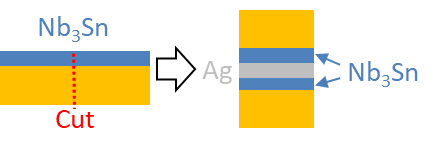
\includegraphics[width=.7\textwidth]{images/Methodology/CuttingCrossSection.png}
        \caption{Schematic of film that is prepared for cross-section by cutting and gluing together using a sandwich structure.}
        \label{fig:CuttingCrossSection}
    \end{figure}
    \FloatBarrier

    When imaged with the polished edge perpendicular to the electron beam, this geometry enables accurate quantitative EDS measurements without angular corrections. However, mechanical stress during cutting can damage brittle films, introduce artifacts such as smearing or pull-out of softer phases, or cause delamination at the film-substrate interface.

    \begin{figure}[H]
        \centering
        
\includegraphics[width=.9\textwidth]{images/Nb/NbsubetchSEM.png}
        \caption{SEM images of a Nb$_3$Sn film on a Nb substrate that was cut in half, and one half was etched and the other half not etched, and sandwiched together.}
        \label{fig:NbsubetchSEM}
    \end{figure}  
    \FloatBarrier
    
    \noindent \textbf{Focused Ion Beam (FIB) milling:} An ion beam mills a trench into the sample, exposing the cross-section in situ with minimal mechanical contact or stress. FIB minimizes damage and provides precise site-specific sectioning, allowing investigation of localized features (defects, grain boundaries). The primary limitation is geometric: standard FIB systems image the milled cross-section at a 52~° stage tilt. For thin films ($\sim500$~nm), this oblique viewing angle causes the electron beam interaction volume to span multiple layers, complicating compositional analysis of the sharp interface.
    
    To overcome the 52~° limitation, a thin lamella ($\sim1-2$~\unit{\um} thick) can be extracted from the cross-section and remounted perpendicular to the electron beam. This lift-out technique positions the film thickness edge-on for direct imaging and perpendicular EDS analysis, eliminating angular artifacts. The thin geometry also reduces electron scattering from material behind the region of interest, improving spatial resolution. If atomic-scale investigation is required, the lamella can be further thinned to electron transparency ($<50$~nm) for transmission electron microscopy (TEM). However, lamella preparation is time-intensive ($2-4$ hours per sample) and was reserved for films exhibiting anomalous features requiring detailed investigation. FIB protocols are detailed in Appendix~\ref{appsec:FIBProtocol}.

    \begin{figure}[H]
        \centering
        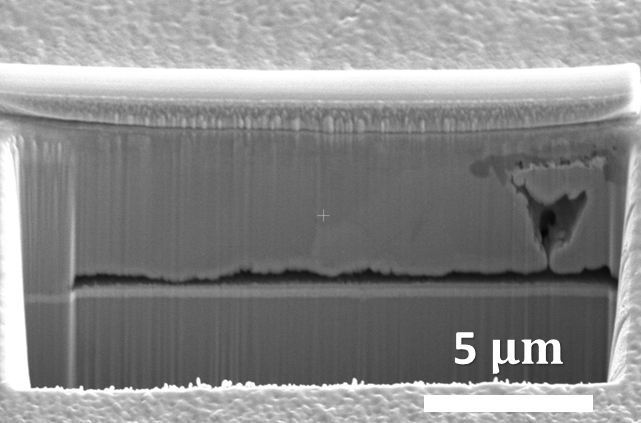
\includegraphics[width=.7\textwidth]{images/Metallurgy/ExampleFIBCrosssection.png}
        \caption{Example FIB cross section SEM image showing voids above the diffusion layer.}
        \label{fig:ExampleFIBCrosssection}
    \end{figure}  
    \FloatBarrier
    

    
    
  
    \subsection{Microscopy and Micro-chemical Analysis}
        
    Film morphology and composition were characterized using scanning electron microscopy (SEM) with energy dispersive spectroscopy (EDS). Visible light microscopy provided initial screening, and transmission electron microscopy (TEM) was used selectively for atomic-scale analysis. Both surface and cross-sectional imaging were performed to correlate microstructural features with RF performance. 
    
    Figure~\ref{fig:FullNb3Sn10micron2} illustrates a typical cross-sectional characterization workflow on a Cu-Sn first sample. The visible light micrograph and SEM image reveal non-uniform surface morphology and thickness variations in the Nb$_3$Sn film, resulting from the underlying bronze layer's porosity and roughness. Multiple Cu-Sn alloy phases near the Nb$_3$Sn surface appear as distinct regions with different contrast. The EDS elemental maps show that Sn penetrated through the Ta diffusion barrier, with comparable Sn concentration on both sides of the Ta layer, indicating barrier failure in this sample. The EDS line scan confirms approximately 25~at.\% Sn uniformly distributed across the film thickness, consistent with stoichiometric Nb$_3$Sn.
        
    \begin{figure}[H]
        \centering
        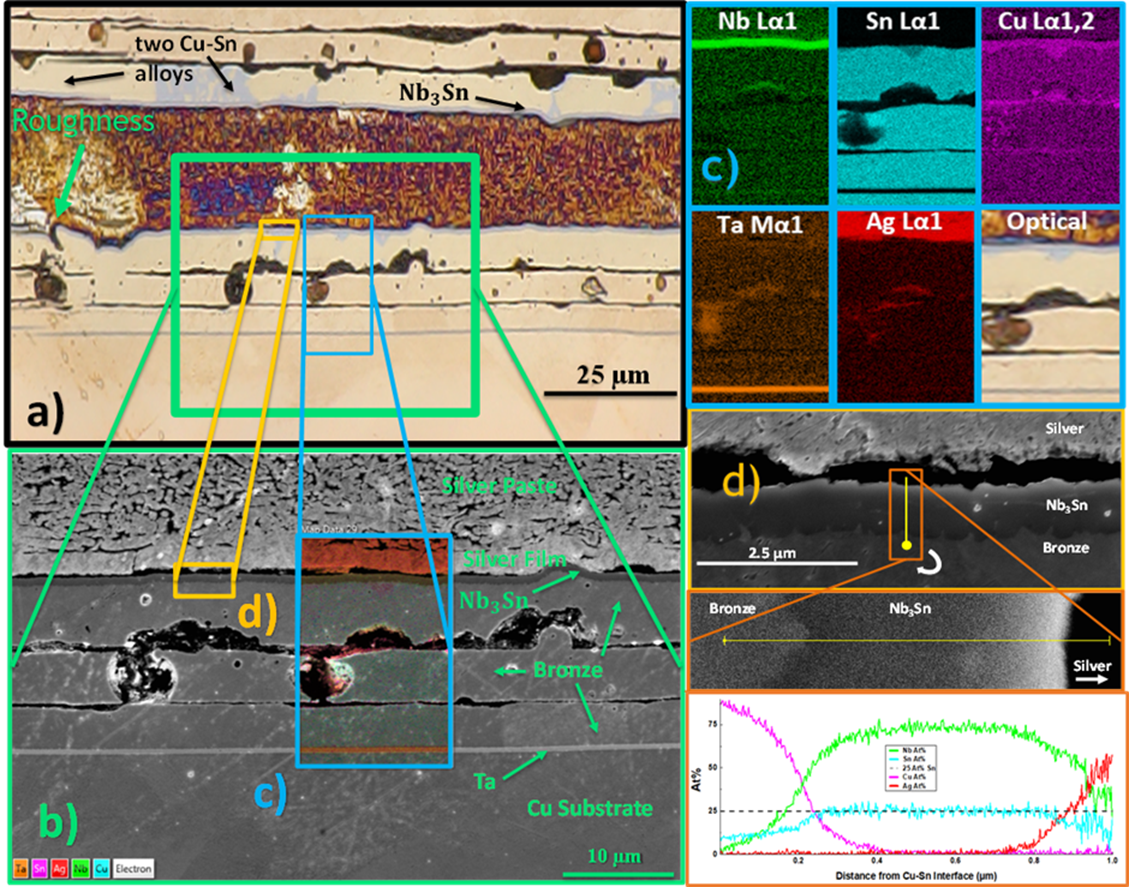
\includegraphics[width=.9\textwidth]{images/Cu/CuSnThickness/FullNb3Sn10micron.png}
        \caption[Cross-sectional characterization of a Cu-Sn first film: (a) visible light micrograph and (b) SEM image showing the layered structure from Cu substrate through Ta barrier, bronze, Nb$_3$Sn, and residual Cu-Sn.]{Cross-sectional characterization of a Cu-Sn first film: (a) visible light micrograph and (b) SEM image showing the layered structure from Cu substrate through Ta barrier, bronze, Nb$_3$Sn, and residual Cu-Sn. Colored boxes indicate regions examined in (c) and (d). (c) EDS elemental maps of the cyan-boxed region. (d) High-magnification SEM and EDS line scan across the Nb$_3$Sn layer (orange-boxed region).}
        \label{fig:FullNb3Sn10micron2}
    \end{figure}
    \FloatBarrier

  \subsubsection{Visible Light Microscopy}
    
    Surface topography and cross-sections were analyzed using an Olympus DSX1000 digital microscope. The instrument constructs three-dimensional surface maps via focus variation, acquiring images at sequential focal planes and computationally stitching in-focus regions. Lateral resolution is diffraction-limited to the wavelength of visible light ($\sim$400--700~nm), but using a 50$\times$ objective, roughness parameters such as $R_a$ can be quantified down to approximately 5~nm. This is sufficient for characterizing substrate roughness before and after deposition.

    \subsubsection{Scanning Electron Microscopy (SEM)}
    
    Scanning electron microscopy uses a focused electron beam to image surface morphology and composition with resolution down to $\sim$5~nm. When the electron beam strikes the sample, it generates multiple signals that provide complementary information:
    
    \begin{itemize}
        \item \textbf{Secondary electrons (SE)}: Emitted from the near-surface region (<10~nm depth), providing high-resolution topographic contrast ideal for imaging grain boundaries, surface roughness, and morphological features
        \item \textbf{Backscattered electrons (BSE)}: Higher-energy electrons scattered from deeper regions ($\sim$100~nm--1~\unit{\um}), providing compositional contrast where heavier elements (higher atomic number Z) appear brighter
        \item \textbf{Characteristic X-rays}: Enable elemental identification and quantification through energy dispersive spectroscopy (described below)
    \end{itemize}
    
    The electron beam is rastered across the sample surface in a grid pattern, and the detected signal intensity at each point creates an image pixel-by-pixel. Unlike visible light microscopy, which is limited by light wavelength to $\sim$200~nm resolution, SEM achieves much finer resolution due to the short de Broglie wavelength of accelerated electrons ($\lambda \sim 0.01$~nm at 10~keV). 
    
    Acceleration voltage selection involves trade-offs: lower voltages (1--5~kV) reduce beam penetration depth, improving surface sensitivity and minimizing charging on insulating samples, while higher voltages (15--30~kV) increase signal generation from deeper regions, excite higher-energy characteristic X-rays from heavy elements, and improve image contrast for thick films. Detailed imaging protocols are provided in Appendix~\ref{appsec:SEMProtocol}.

    \subsubsection{Energy Dispersive Spectroscopy (EDS)}
        
    Energy dispersive spectroscopy (EDS) analyzes characteristic X-rays emitted when the electron beam excites inner-shell electrons in the sample. When an inner-shell electron is ejected, an outer-shell electron fills the vacancy, releasing an X-ray with element-specific energy.
        
    Figure~\ref{fig:EDSSpectrum} shows EDS spectra from two locations on a Nb$_3$Sn film. The detector sorts X-rays by energy, producing a histogram of counts versus keV. Each peak corresponds to a characteristic transition: Nb~L$\alpha$1 at 2.17~keV, Sn~L$\alpha$1 at 3.44~keV, and Cu~K$\alpha$1 at 8.04~keV. Spectrum~1, from a Nb-rich region, shows strong Nb, Sn, and Cu peaks; Spectrum~2 from the surrounding matrix is predominantly Cu.
        
    EDS provides three measurement modes~\cite{AZtecUserManual2023}:
        
    \textbf{Point analysis} acquires a spectrum from a stationary beam position, typically dwelling 30--120~seconds. The analyzed volume is approximately 1~\unit{\um}$^3$ at 15--20~kV.
        
    \textbf{Line scans} acquire spectra sequentially along a path, stepping point-to-point with 0.1--1~s dwell times. This produces compositional profiles useful for measuring gradients across interfaces or layered structures.
        
    \textbf{Elemental mapping} rasters the beam across a region, collecting X-rays at each pixel. The system defines energy ``windows" around peaks of interest. Figure~\ref{fig:EDSSpectrum} shows Cu, Nb, and Sn maps from the same region as the point spectra. Map acquisition typically requires 30 minutes to several hours.
    
    Quantitative accuracy is $\sim$1--2~at.\% for elements with Z $\geq$ 11. Light elements (Z $<$ 11) produce weak signals due to low fluorescence yield.


    %\subsubsection{Energy Dispersive Spectroscopy (EDS)}
    
    %Energy dispersive spectroscopy (EDS) analyzes characteristic X-rays emitted when the electron beam excites inner-shell electrons in the sample. When an inner-shell electron is ejected, an outer-shell electron fills the vacancy, releasing energy as an X-ray photon. The X-ray energy is element-specific (determined by the atomic electron binding energies), creating a unique elemental ``fingerprint".
    
    %Figure~\ref{fig:EDSSpectrum} shows representative EDS spectra acquired from two locations on a Nb$_3$Sn film on a Nb substrate covered with Cu-Sn. The detector counts incoming X-rays and sorts them by energy, producing a histogram of counts versus energy (in keV). Each peak corresponds to a characteristic X-ray transition: for example, Nb~L$\alpha$1 at 2.17~keV, Sn~L$\alpha$1 at 3.44~keV, and Cu~K$\alpha$1 at 8.04~keV. Peak identification enables qualitative analysis, while peak integration (after background subtraction) provides quantitative atomic percentages. Spectrum~1, acquired from a Nb-rich region, shows strong Nb, Sn, and Cu peaks, whereas Spectrum~2 from the surrounding matrix is predominantly Cu.
    
    %EDS provides three primary measurement modes, each building on the same X-ray detection principle~\cite{AZtecUserManual2023}:
    
    %\textbf{Point analysis} acquires a spectrum from a stationary beam position. The electron beam dwells at a single location while the detector accumulates X-ray counts, typically for 30--120~seconds depending on the required statistical precision. Longer acquisition times improve peak-to-background ratios and reduce quantification uncertainty. The electron-interaction volume determines the analyzed volume, approximately 1~\unit{\um}$^3$ at 15--20~kV, implying that the composition represents an average over this region.
    
    %\textbf{Line scans} acquire spectra sequentially along a defined path across the sample. The beam steps from point to point along the line, dwelling briefly (0.1--1~s) at each position to collect a spectrum. The software extracts the intensity of selected elemental peaks at each point, producing a compositional profile. Line scans are beneficial for measuring concentration gradients across interfaces or through layered film structures.
    
    %\textbf{Elemental mapping} extends this concept to two dimensions. The beam raster scans across a rectangular region, and at each pixel, the detector collects X-rays. Rather than storing full spectra, the system defines energy ``windows" centered on characteristic peaks of interest---for example, a window spanning 2.0--2.3~keV captures Nb~L$\alpha$ X-rays while excluding other elements. The X-ray counts within each window are recorded as a function of beam position, generating a spatial map of elemental distribution. Figure~\ref{fig:EDSspectrum}(c) shows elemental maps for Cu, Nb, and Sn acquired from the same region as the point spectra, illustrating how the Nb-rich and Cu-rich phases visible in the SEM image correspond to distinct compositional domains. Map acquisition requires extended dwell times at each pixel to accumulate sufficient counts, typically 30~minutes to several hours, depending on the desired resolution and signal strength. Quantitative accuracy is limited to $\sim$1--2~at.\% for elements with Z $\geq$ 11 (Na and heavier). Light elements (Z $<$ 11) produce weak signals due to low fluorescence yield and strong absorption.
    
    \begin{figure}[H]
        \centering
        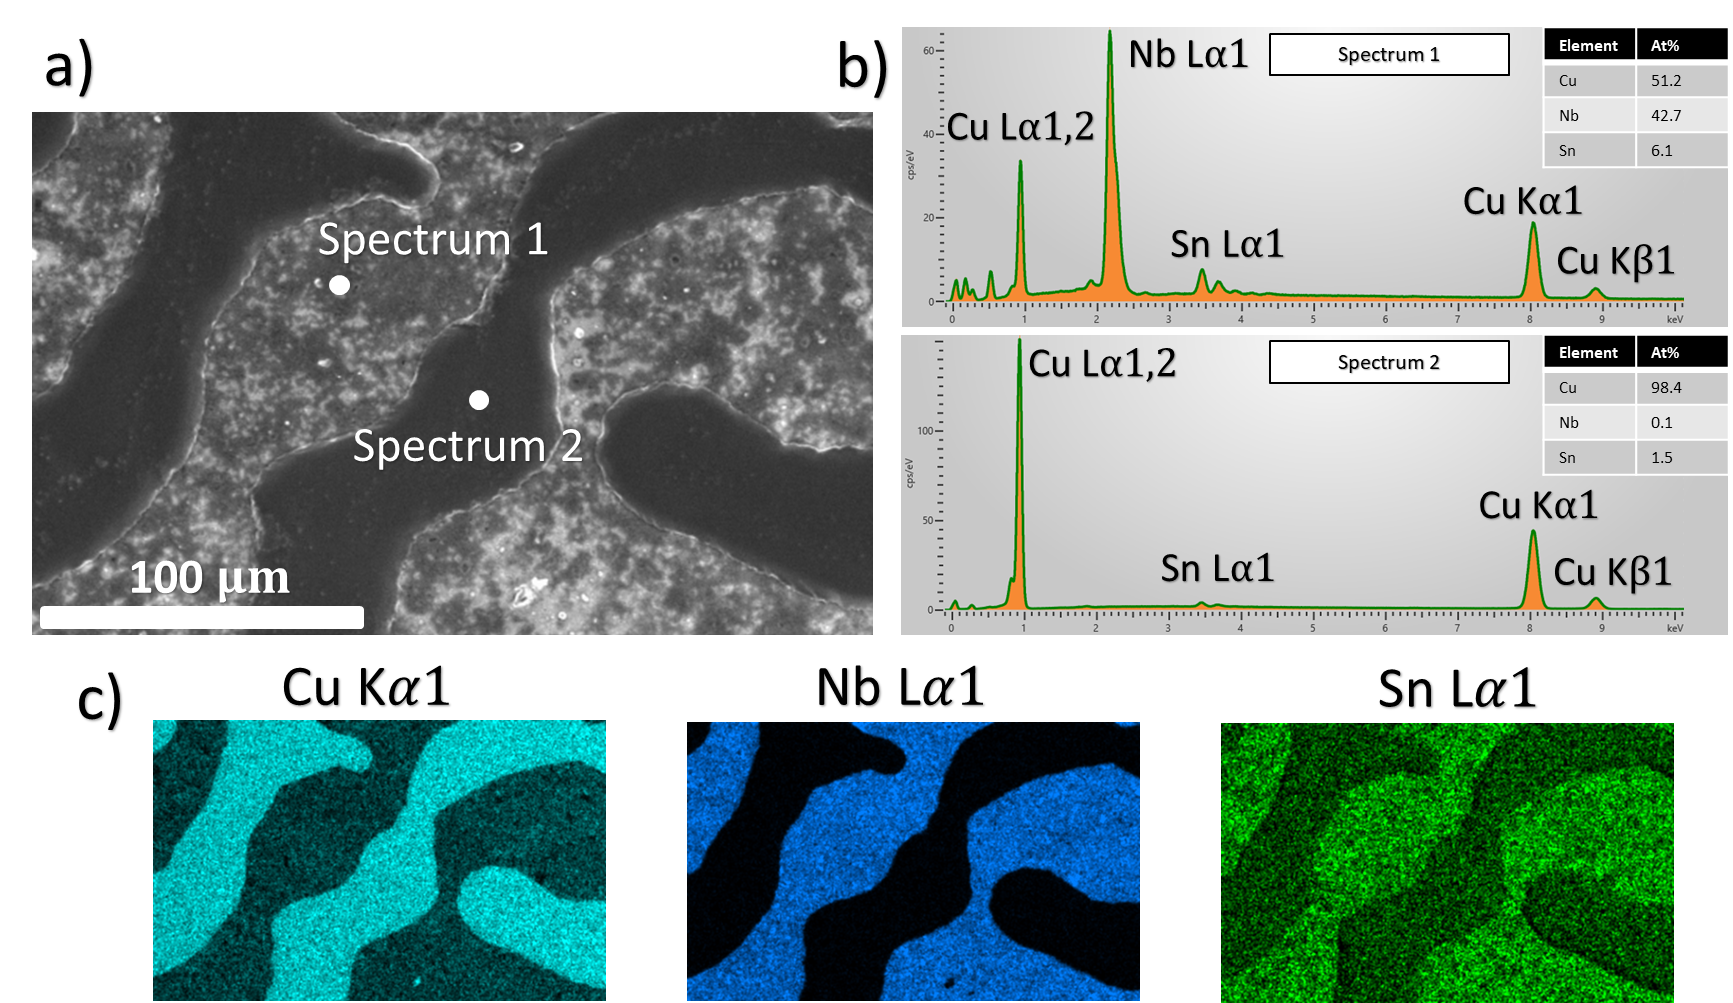
\includegraphics[width=.9\textwidth]{images/Metallurgy/EDSSpectrum.png}
        \caption{SEM image (a) with (b) EDS point scan and (c) EDS mapping showing elemental content in different regions.}
        \label{fig:EDSSpectrum}
    \end{figure}
    \FloatBarrier
    
\section{Critical Temperature Measurements}\label{sec:TcDetail}
    
    \subsection{SQUID Magnetometry}
    
    \subsubsection{Operating Principle}
    
    Traditional AC susceptometry measurements measure a change in magnetic flux:
    
    \begin{equation}
    V = \frac{d\Phi}{dt}
    \end{equation}
    
    \noindent where $\Phi$ is the flux contained in the coil. However, in a SQUID system, the output voltage is proportional to the magnetic flux in the pick-up coil instead of its time derivative. The measurement involves quantization in superconducting loops. As a sample is moved within the area enclosed by a superconducting loop, a persistent screening current is induced and coupled through a transformer to a Josephson junction that detects flux changes with extreme sensitivity.
    
    Multiple loops comprising four superconducting coils, wound in a counterwound configuration (two clockwise, two counterclockwise), form a second-order gradiometer that rejects uniform field flux while detecting local moments. Therefore, if a homogeneous sample is longer than the distance between the outer loops, the magnetic moment is counted as a uniform external field and is not measured. For this reason, samples must be small ($<10$~mm).
    
    \begin{figure}[tb]
        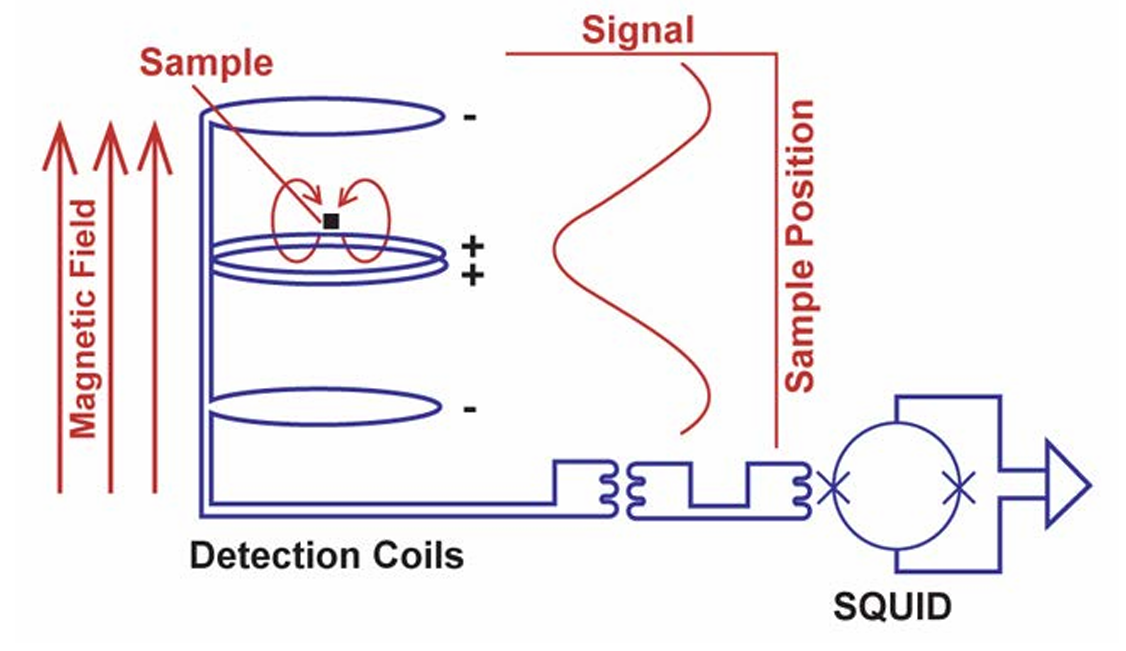
\includegraphics[width=.8\textwidth]{images/Methodology/SQUID.png}
        \centering
        \caption{Superconducting Quantum Interference Device (SQUID) schematic showing sample translation through pickup coils and Josephson junction detection \cite{designquantumMagneticPropertyMeasurement2009}.}
        \label{fig:SQUID}
    \end{figure}

    The sample is mounted on a long plastic straw that cannot be magnetized. The straw is continuous along the entire sample path, ensuring the coils experience no change in flux due to the straw. As the magnetized sample moves through the detection coils (Fig.~\ref{fig:SQUID}), the magnetic flux $\Phi = BA$ is felt by the coils, where $B = \mu_0(H + M)$. The pick-up coils are wound such that a material that increases the enclosed $B$ (i.e., $M > 0$ for $H > 0$) produces a positive voltage, while a diamagnetic response ($M < 0$) produces a negative voltage. Since the voltage amplitude is proportional to the magnetic moment, small-volume samples require high magnetization to produce a measurable signal.

    Magnetized samples can be characterized into three groups based on their response to an applied magnetic field (Fig.~\ref{fig:FluxResponseInMaterials}). A superconductor exhibits a diamagnetic response where $M = -H_0$, expelling the applied field from its interior so that $B = 0$ inside the bulk. A ferromagnet exhibits a strong positive magnetization $M \gg H_0$, greatly increasing the flux density inside the material. An insulator or weakly magnetic material exhibits a paramagnetic response where $M \approx 0$, producing a small positive change in the local flux density.

    These different magnetic responses produce characteristic voltage curves as the sample translates through the gradiometer pickup coils (Fig.~\ref{fig:SQUIDScanSimulate}). For the counterwound coil configuration ($-1, +2, -1 $), a diamagnetic sample that reduces the local flux density produces a curve with a central negative peak. A ferromagnetic sample that increases the local flux density produces a curve with a central positive peak of larger amplitude. A paramagnetic sample produces a curve similar in shape to the ferromagnet but with much smaller amplitude, reflecting its weak magnetic response. The amplitude of the voltage curve is proportional to the sample's magnetic moment, and the software fits the curve to extract the magnetic moment.
    
    \begin{figure}[tb]
        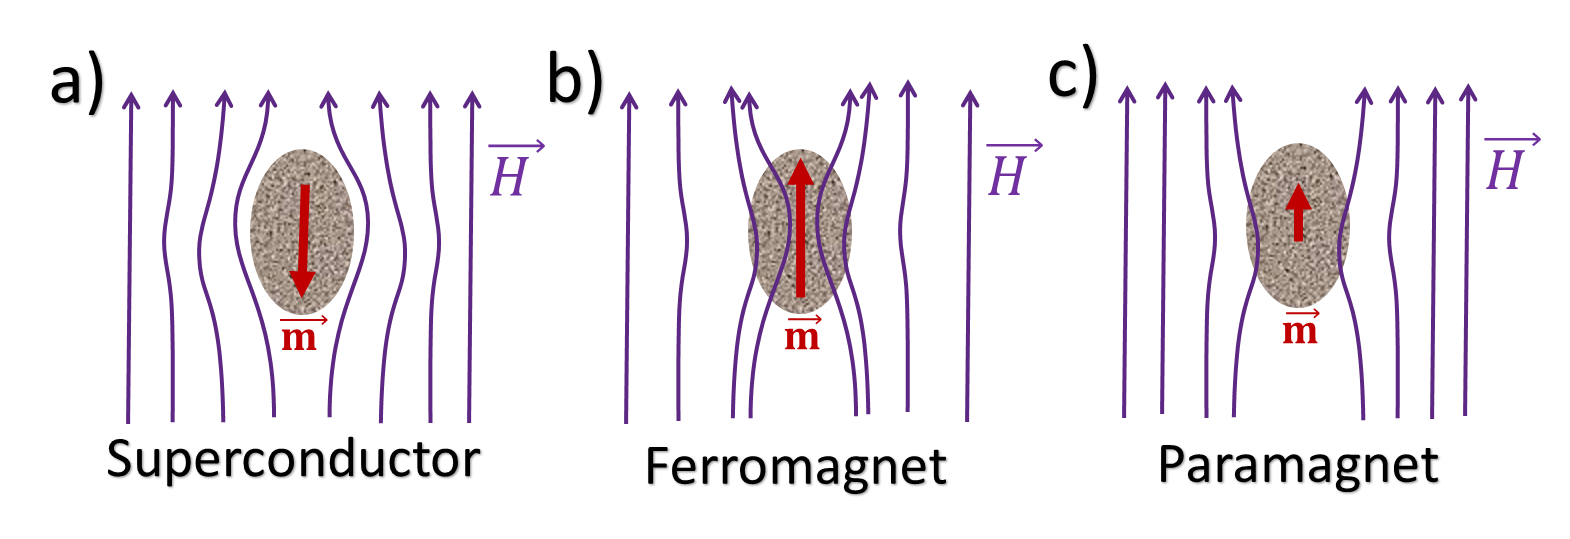
\includegraphics[width=\textwidth]{images/Methodology/FluxResponseInMaterials.png}
        \caption{Ideal flux response to a small magnetic field for different samples: a) superconductor, b) ferromagnet, and c) paramagnet.}
        \label{fig:FluxResponseInMaterials}
    \end{figure}
    
    \begin{figure}[tb]
        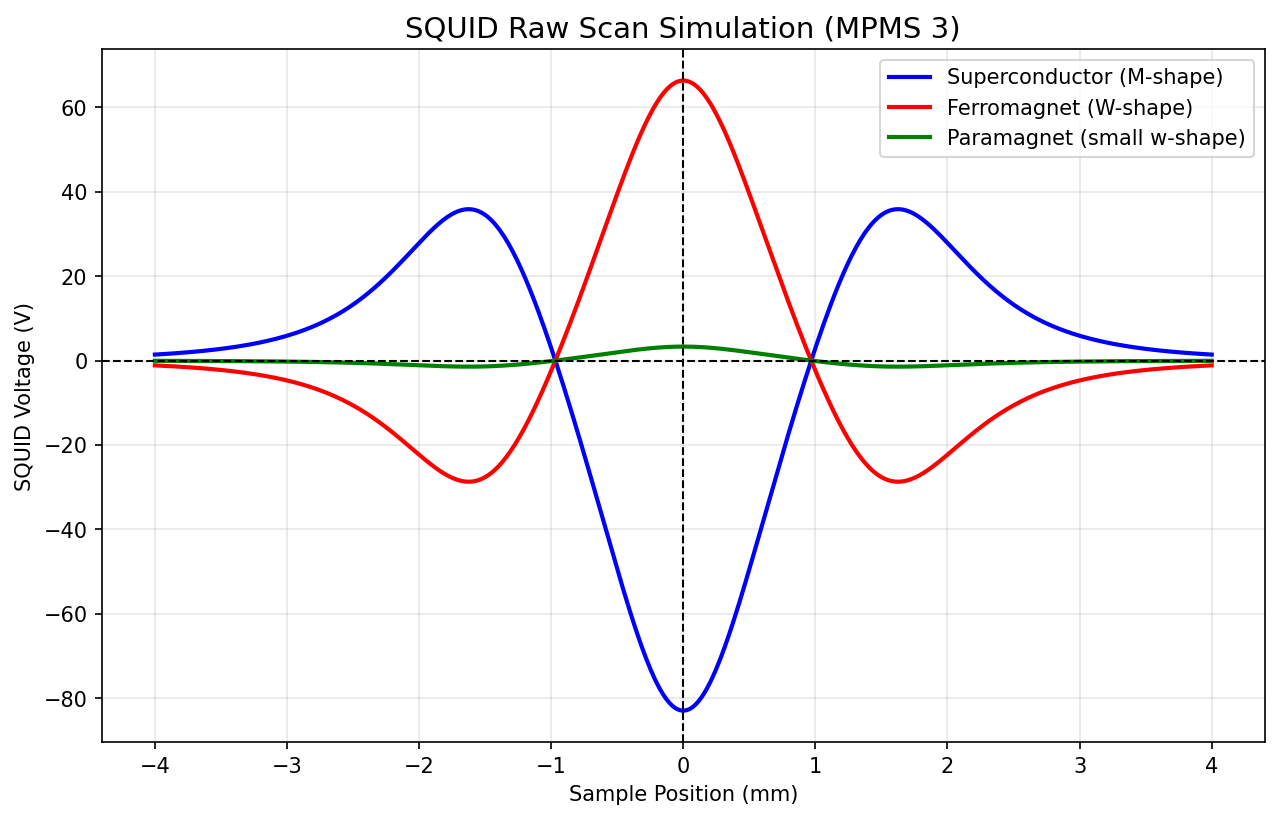
\includegraphics[width=\textwidth]{images/Methodology/SQUIDScanSimulate.png}
        \caption{Simulated SQUID scans for superconductor, ferromagnet, and paramagnet, when coil is in -1, +2, -1 set up.}
        \label{fig:SQUIDScanSimulate}
    \end{figure}
    
    \subsubsection{Instrumentation}
    
    Temperature in the MPMS is controlled via helium gas flow through a copper heat exchanger with resistive heating elements, regulated by PID feedback. Magnetic fields are generated by a persistent-mode superconducting solenoid.
    
    \subsubsection{Measurement Protocol}
    
    The voltage-to-magnetic moment conversion is standardized using a palladium (Pd) sample. Since the Bohr magneton per atom at $T = 0$, density of Pd, mass of sample, and number of atoms $N = m N_A / A_w$ are known, the theoretical magnetic moment $m_{\text{theory}} = 0.6 \mu_B N$ can be calculated. The standard sample is compared to theory, and a calibration factor is applied. The Pd sample can achieve accuracy within 0.1\% for a point-dipole geometry~\cite{quantumdesigninc.MPMS3Users2016}. With this calibration, any future voltage measurement can be converted to a magnetic moment. Magnetic moment $m$ has units of A\,m$^{2}$, where 1~emu $= 10^{-3}$~A\,m$^{2}$. If the volume of the thin film is known, the total magnetization $M$ can be calculated given $m = \int M \, dV$. Often, the volume is unknown, so the normalized magnetic moment is plotted.
    
    The sample must be centered along the length of the superconducting coils so the magnetic moment can be measured appropriately. Zero-field-cooled (ZFC) measurements are the standard measurement technique for reducing trapped flux and maximizing magnetic moment. The trapped field in the superconducting magnet is minimized by oscillating the magnetic field from positive to negative values as it approaches zero, called degaussing. The residual field can be further reduced by measuring the sample's magnetic moment as a function of the magnetic field. While the sample is below $T_c$, the magnetic field is set to a small negative value ($-1$~Oe), and ramped to a positive value ($+1$~Oe) in small steps. The point at which the line crosses the x-axis indicates the actual zero magnetic field value experienced by the sample. This is typically between $-1$ and $+1$~Oe if degaussing is done correctly. This zero value is the new zero-field value and must be used as a correction for the rest of the measurement. If trapped flux is not removed from the sample, the sample exhibits a smaller magnetic moment and may transition faster depending on the impurity concentration.
    
    For thin-film samples, demagnetization effects can be minimized by applying the field parallel to the thin-film surface. Specific measurement protocols are detailed in Appendix~\ref{appsec:SQUIDProtocol}.
    
    \subsection{Superconductor Response}
    
    \subsubsection{Bulk Samples}
    
    When a superconductor perfectly expels a magnetic field from the bulk ($B = 0$), as in the Meissner state, the magnetization $M \approx -H_0$. This gives the maximum negative magnetic moment, $m = -1$ when normalized. Even when the superconductor is not perfectly in the Meissner state, the sample exhibits a diamagnetic response. The screening currents, as discussed in Sec.~\ref{sec:superconductor}, are induced perpendicular to the external magnetic field to expel the magnetic field from the bulk, setting $B = 0$. If the sample thickness is much larger than the penetration depth, $d \gg \lambda$, the superconductor perfectly screens the external magnetic field, and the magnetic moment is maximized. As temperature increases, $\lambda$ gets larger, but as long as $\lambda \ll d$, perfect diamagnetic response continues.
    
    As the temperature increases, the areas of the sample with poor superconducting properties transition from diamagnetic (large negative $M$) to paramagnetic (small positive $M$), when $T>T_c$. This shift from superconducting to non-superconducting occurs very rapidly in uniform samples and very gradually in non-uniform films. This transition continues until the entire sample becomes diamagnetic, and all areas have reached their respective critical temperatures. A schematic explaining the change in magnetic moment with temperature and the resulting critical temperature curve is given in Fig.~\ref{fig:MomentvsTempLance}. If the sample is divided by cracks or has polluted grain boundaries, the magnetic field can penetrate intergranularly, thereby reducing the magnetic moment. 

    \begin{figure}[H]
        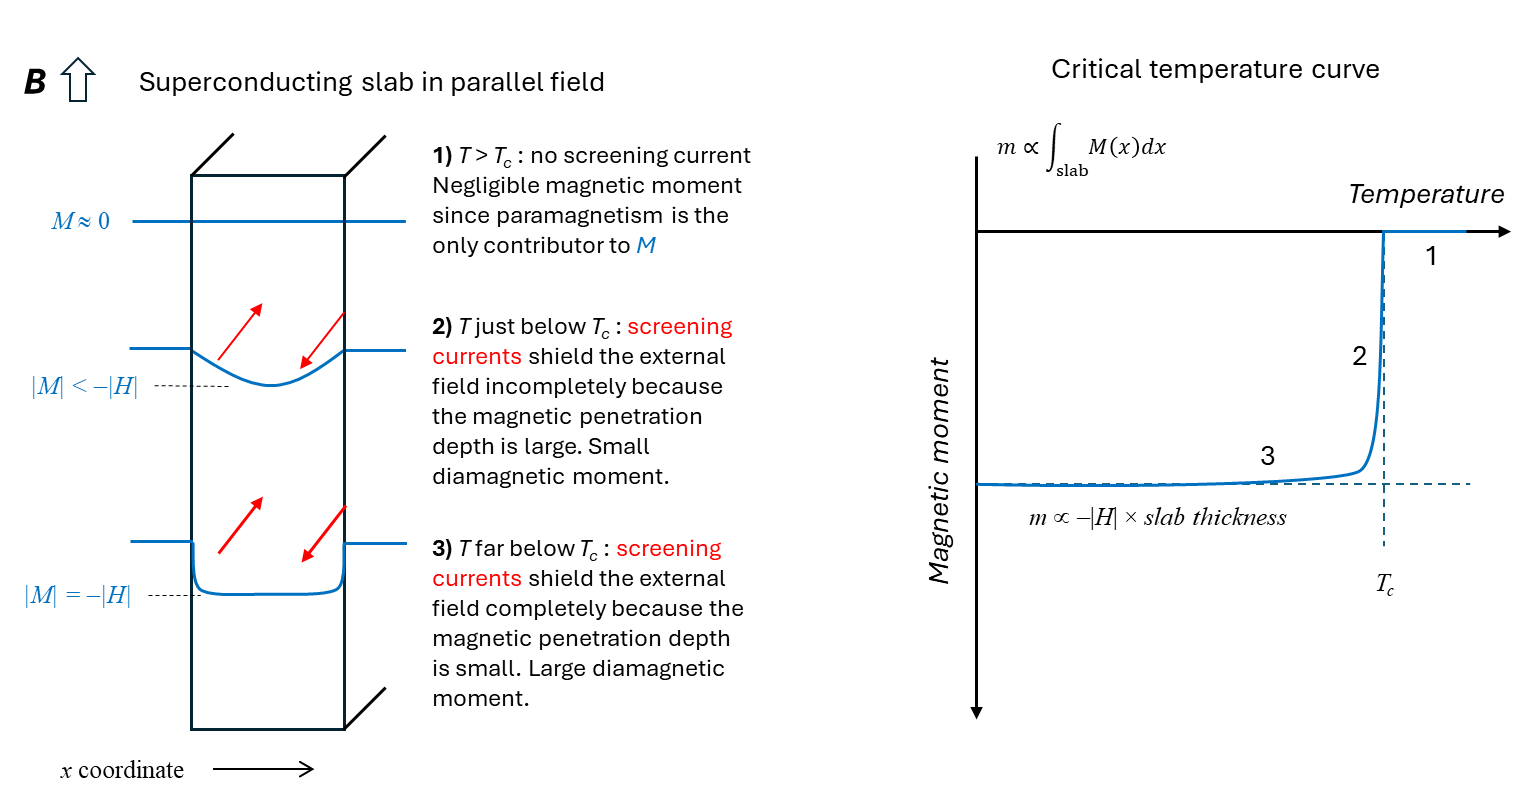
\includegraphics[width=\textwidth]{images/Methodology/MomentvsTempLance.png}
        \caption{Superconducting slab in parallel field with example critical temperature curve}
        \label{fig:MomentvsTempLance}
    \end{figure}
    
    \subsubsection{Thin Films}
    
    If the superconducting material has a thickness on the same order as the penetration depth, $d \sim \lambda$, the magnetic field cannot be perfectly screened. The material is still diamagnetic but has a smaller magnetic moment $|M| < H_0$ (seen in Fig.~\ref{fig:MagnetizationofDifferentGeometries}). As the temperature increases, more and more of the material is ineffectively screened even if the sample is perfectly uniform, resulting in a decreasing magnetic moment. This appears as a transition width even in uniform films.
    
    \begin{figure}[tb]
        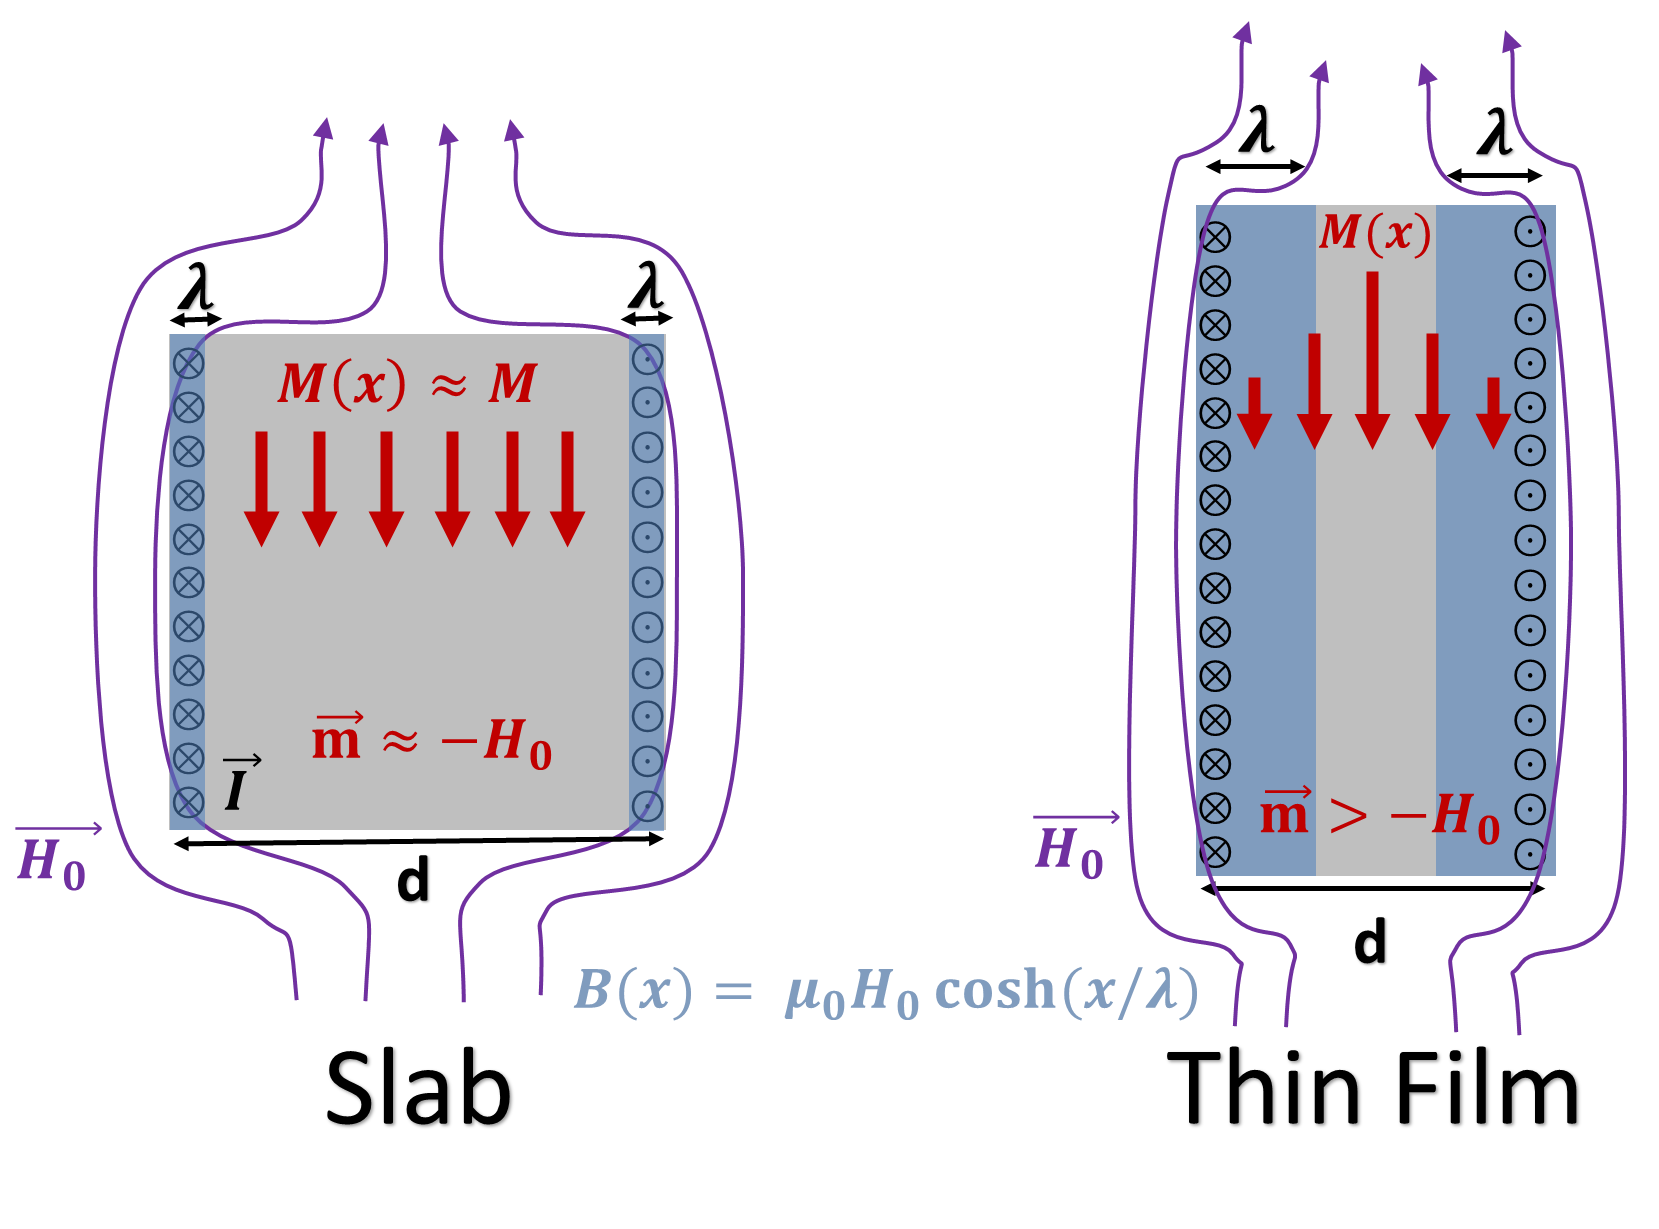
\includegraphics[width=\textwidth]{images/Methodology/MagnetizationofDifferentGeometries.png}
        \caption{Magnetization of large samples where $d \gg \lambda$ and thin films where $d \sim \lambda$.}
        \label{fig:MagnetizationofDifferentGeometries}
    \end{figure}

    For example, consider Nb$_3$Sn with $\lambda \approx 100$~nm. In a 1~mm-thick bulk sample, the field penetrates only $\sim$200~nm total (100~nm from each surface parallel to external field), representing 0.02\% of the volume, the interior is fully screened and the sample exhibits near-ideal diamagnetism. In a 300~nm thin film, however, the field penetrates approximately 2/3 of the thickness, significantly reducing the diamagnetic moment. The reduced moment arises not only from the smaller volume but also from incomplete screening throughout the film.

    Sample geometry also affects the apparent critical field. Flux lines bend around a superconductor and concentrate at edges and corners, increasing the local field relative to the applied field. This demagnetization effect causes flux to penetrate edges at lower applied fields than would penetrate a flat parallel surface. A prolate spheroid with its long axis parallel to the field minimizes this effect, yielding nearly uniform flux penetration (Fig.~\ref{fig:Demag}a). A thin film oriented perpendicular to the field maximizes edge effects, causing early flux penetration at the edges (Fig.~\ref{fig:Demag}b). Orienting the film parallel to the field significantly reduces demagnetization (Fig.~\ref{fig:Demag}c); this geometry was used for all measurements in this work. Nevertheless, demagnetization complicates accurate determination of the lower critical field $H_{c1}$.
    
    \begin{figure}[H]
        \centering
        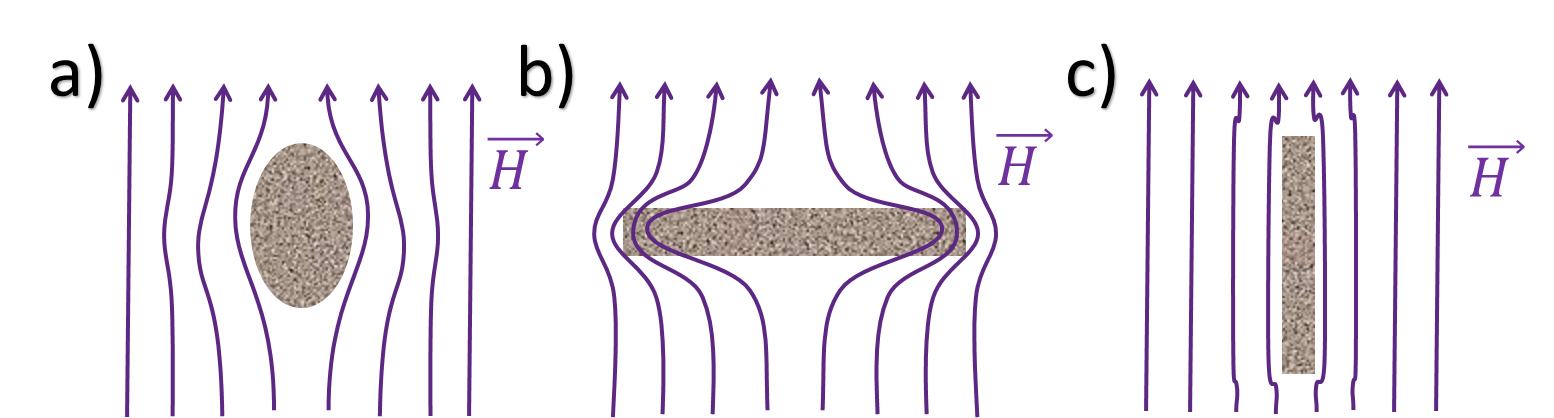
\includegraphics[width=\textwidth]{images/Superconductor/Demag.png}
        \caption[Demagnetization affecting magnetic field penetration at the edges for (a) spheroid and (b,c) thin film geometries.]{Demagnetization affecting magnetic field penetration at the edges for (a) spheroid and (b,c) thin film geometries. Perpendicular field orientation (b) maximizes edge effects, while parallel field orientation (c) minimizes edge effects in thin films. Parallel field orientation was used for all measurements.}
        \label{fig:Demag}
    \end{figure}
    
    \subsubsection{Interpretation of $T_c$ Curves}
    
    The $T_c$ transition provides diagnostic information about film quality. As the sample is heated from low temperature (2~K), regions with lower critical temperatures transition to the normal state, while higher-quality regions transition to normal state at temperatures close to maximum $T_c$. The critical temperature of Nb$_3$Sn depends on local variations in strain and Sn content, with zero strain and stoichiometric composition giving the highest $T_c$ (see Sec.~\ref{sec:Tceffectch5}). Film properties vary along the thickness. The transition width of the critical temperature curve reflects this variation, while the $T_c$ onset indicates the strain and Sn content in the highest-quality regions. High-$T_c$ regions can magnetically shield low-$T_c$ regions, complicating interpretation (see Sec.~\ref{sec:SapphireExp}). This effect is illustrated schematically in Fig.~\ref{fig:SnandStrainCriticalTempLance}. As temperature increases, less of the sample becomes diamagnetically screened, uncovering the magnetic response from low-Sn and high-strain regions.

    \begin{figure}[H]
        \centering
        
\includegraphics[width=\textwidth]{images/Methodology/SnandStrainCriticalTempLance.png}
        \caption{Schematic of superconducting slab with variable Sn or strain properties}
        \label{fig:SnandStrainCriticalTempLance}
    \end{figure}
    
    Figure~\ref{fig:TcExplanation} shows $T_c$ curves for two Nb$_3$Sn films on Cu substrates. The black curve exhibits a sharp transition ($\Delta T_c \approx 0.6$~K), indicating high compositional uniformity, while the red curve shows a broader transition due to a wider range of Sn concentration. The higher $T_c$ onset in the red curve is attributed to strain relaxation in the thicker film. Secondary transitions at 6~K and 8~K indicate additional phases, likely Sn-rich intermetallics or unreacted Nb. Because of the interrelated effects of strain and composition on the critical temperature, we rely on theory and other experimental methods to further characterize the sample. However, this measurement provides rapid screening of superconducting film quality before proceeding to more time-intensive characterization.
    
    \begin{figure}[H]
        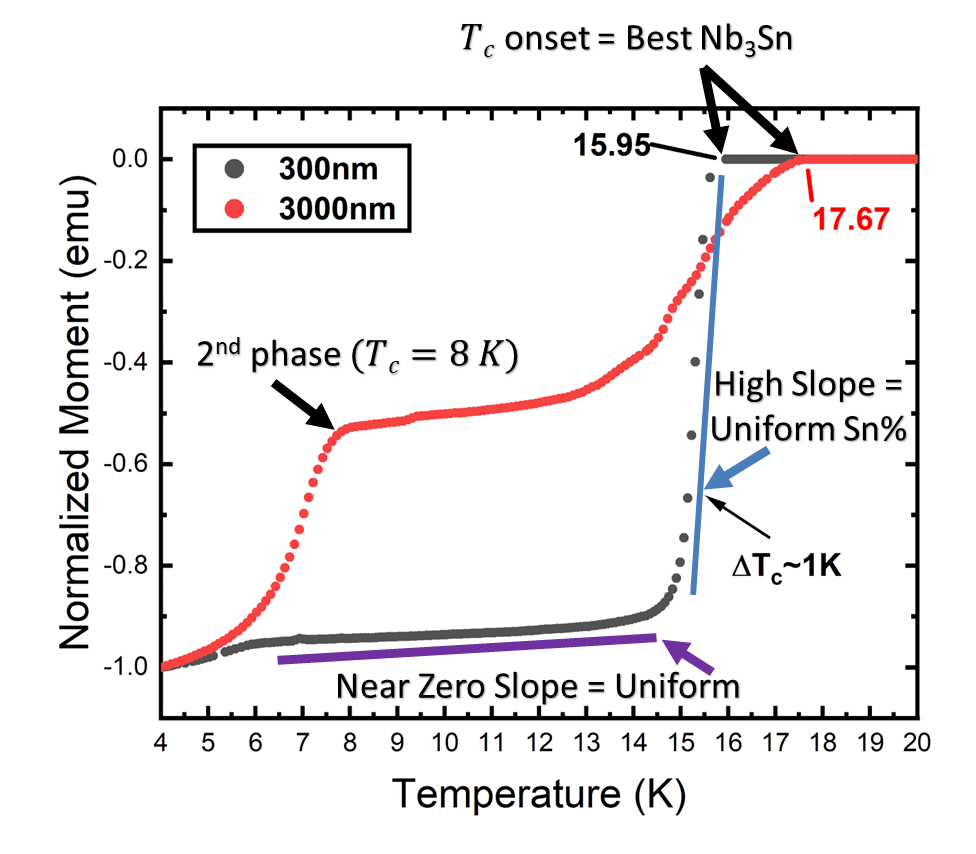
\includegraphics[width=\textwidth]{images/Methodology/TcExplanation.png}
        \caption[Critical temperature curves for two Nb$_3$Sn samples on Cu substrates.]{Critical temperature curves for two Nb$_3$Sn samples on Cu substrates. The black curve exhibits a sharp transition ($\Delta T_c \approx 0.6$~K) with $T_c$ onset at $\approx 16$~K. The red curve shows a broader transition with a higher $T_c$ onset. Secondary transitions at 6~K (black) and 8~K (red) indicate additional phases.}
        \label{fig:TcExplanation}
    \end{figure}



\section{RF Characterization of Pillbox Cavities}
    
    \subsection{Measurement Principles and Instrument Configuration}
    To characterize the RF properties of copper and determine its surface resistance, the material is fabricated into a cylindrical "pillbox" cavity. This common geometry is often used because it can be solved analytically easily, enabling comparison among simulation, theory, and experiment.
    
    The fundamental instrument for these measurements is the Vector Network Analyzer (VNA). The VNA serves as a phase-coherent source and receiver, facilitating S-parameter measurements. In a two-port configuration:
    \begin{itemize}
        \item \textbf{Transmission ($S_{21}$):} Measures power delivered from Port 1 to Port 2 through the cavity.
        \item \textbf{Reflection ($S_{11}$):} Measures power reflected from Port 1 back to Port 1.
    \end{itemize}
    
    These S-parameters are frequency dependent. When a circuit component (cavity) has a resonant frequency equal to the stimulating AC frequency, the transmitted signal is resonantly enhanced. This signal peak occurs because the power is resonantly enhanced by the cavity walls when the input AC frequency is in resonance with the cavity mode. The frequency locations of the resonance modes for the cavity geometry are already known using simulation (Sec.~\ref{sec:cavitydesign}). The VNA is set to these frequencies to check for resonant behavior. The measurement circuit is impedance-matched to 50~$\Omega$. While the coaxial shields are grounded via the VNA chassis, the cavity enclosure must be connected to a common ground to suppress external electromagnetic interference. The PPMS, probe design, VNA, and cavity used are shown in Fig.~\ref{fig:ProbePPMSVNACavity}.
    
    
    \begin{figure}[H]
        \centering
        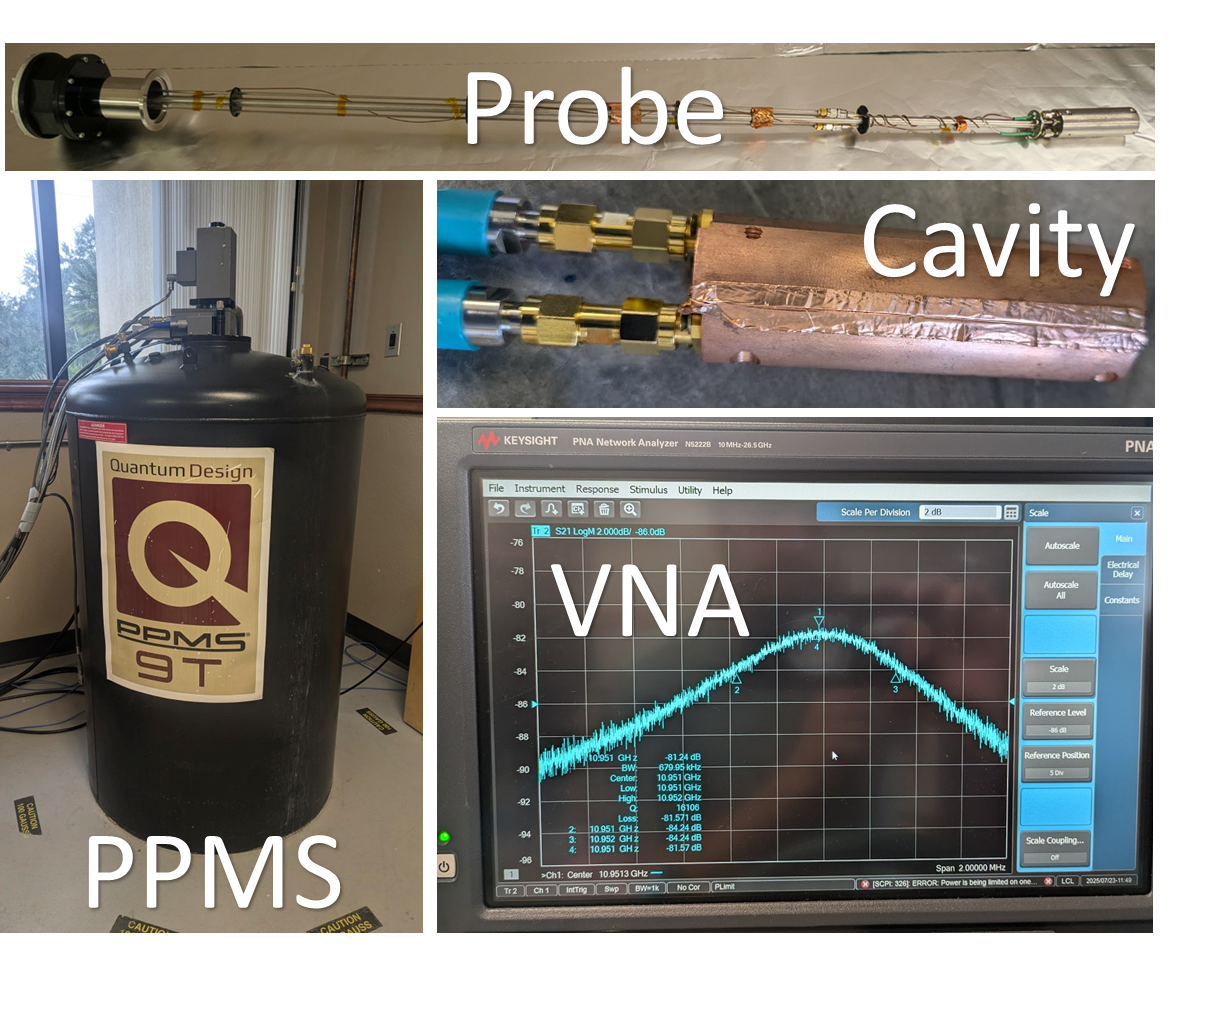
\includegraphics[width=0.9\linewidth]{images/AndreCavity/ProbePPMSVNACavity.png}
        \caption{Experimental apparatuses needed for Q measurement: probe~\cite{Braine:2024nzi}, PPMS magnet, cavity, and VNA.}
        \label{fig:ProbePPMSVNACavity}
    \end{figure}
    
    
    When transitioning from room temperature to cryogenic environments, the conductivity of copper increases, leading to a significant rise in $Q_0$. Lowering the temperature also reduces skin depth, allowing current to navigate through even smaller gaps. However, at 10~GHz, the surface resistance reaches a limit defined by the Anomalous Skin Effect, where the electron mean free path exceeds the skin depth. Furthermore, thermal contraction of the copper reduces the cavity dimensions, shifting $f_0$ to higher frequencies. These shifts can be tracked in real-time.
    
    \subsection{Determining the Quality Factor of an Ideal Cavity}
    
    The Quality Factor ($Q$) represents the ratio of energy stored in the cavity to the energy dissipated per cycle. Three $Q$ values can be distinguished: the loaded ($Q_L$), the external ($Q_{ext}$), and the intrinsic ($Q_0$).
    
    \subsubsection{Loaded Quality factor $Q_L$}
    $Q_L$ is extracted from the $S_{21}$ transmission peak by measuring the resonance frequency ($f_0$) and the 3~dB full-width at half-maximum ($\Delta f_{3dB}$):
    \begin{equation}
        Q_L = \frac{f_0}{\Delta f_{3dB}}
        \label{eq:QVNA_fixed}
    \end{equation}
    \noindent A narrower peak signifies a higher $Q$, indicating lower surface resistance in the copper walls.
    
    \subsubsection{Intrinsic $Q_0$}\label{sec:Qantenna}
    The antennas used to probe the cavity introduce their own losses and must be accounted for to isolate the material-dependent intrinsic quality factor ($Q_0$) using the coupling coefficients $\beta_1$ and $\beta_2$:
    
    \begin{equation}
        Q_0 = Q_L (1 + \beta_1 + \beta_2)
        \label{eq:Q0_calculation}
    \end{equation}
    
    \noindent The coupling coefficients can be calculated from:
    
    \begin{equation}
        \beta = \frac{1 + \text{sign}(\angle\Gamma(f_0) - \pi)|\Gamma(f_0)|}{1 - \text{sign}(\angle\Gamma(f_0) - \pi)|\Gamma(f_0)|}~.
        \label{eq:beta}
    \end{equation}
    
    \noindent where $|\Gamma|$ the reflection coefficient and its phase $\angle\Gamma$ is another name for the S-parameter. The sign function indicates whether the antenna is over-coupled or under-coupled to the cavity mode, as determined by the phase of the reflection coefficient relative to $\pi$ radians. Practically, $\beta$ is a measure of the depth of the dip from the reflection measurements on resonance. 
    
    In this work, "weak coupling" is used, in which antenna penetration is minimized until the reflection dips are $<1$~dB. The antenna penetration depth can be adjusted by trimming or pulling the antennas out of the cavity. Strong coupling (deep antenna penetration) heavily loads the cavity, presenting a low impedance that reflects significant power and degrades $Q$. Weak coupling (shallow penetration) minimally perturbs the cavity's resonance while maintaining sufficient signal for measurement. When the reflection dip is less than 1~dB, the antenna interacts minimally with the cavity, and the reduction in the antenna's quality factor is also minimal (<5\% loss in $Q$ per antenna). For example, if $Q_L$ is measured to be 100,000, and reflection dips $S_{11}$ and $S_{22}$ are about 1~dB deep on resonance, $Q_0$ will be about 110,000. For initial prototyping, a 10\% reduction in $Q$ is considered negligible, so, for simplicity, we set $Q_L = Q_0$.
    
        \begin{figure}[H]
            \centering
            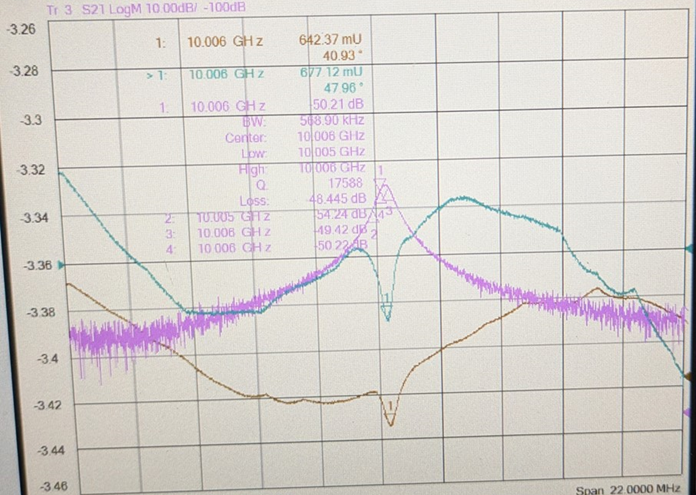
\includegraphics[width=.75\textwidth]{images/AndreCavity/CouplingExample.png}
            \caption[Example vector network analyzer scan for a specific mode at 10 GHz.]{Example vector network analyzer scan for a specific mode at 10 GHz. The purple curve shows the transmission measurement $S_{21}$ or $S_{12}$, and the quality factor can be read from the 3 dB full-width at half-maximum of the peak. The blue and yellow curves show the reflection measurements $S_{11}$ and $S_{22}$, and the coupling from the antenna to the cavity can be inferred from the depth of the dip. A dip of less than 1 dB from background to trough is adequate.}
            \label{fig:CouplingExample}
        \end{figure}
        
        It should be noted that different modes will couple differently to the antenna. For example, specific modes may isolate the current away from the antenna, leading to reduced coupling. 
    

    \subsection{Quality Factor Correction for Hybrid Material Cavities with RF Leakage}\label{sec:QHybrid}

    When characterizing a superconducting coating deposited on only a portion of a copper cavity, the measured quality factor reflects contributions from both materials. Additionally, multi-piece cavity assemblies exhibit RF leakage at mechanical seams. To extract the intrinsic surface resistance of the superconducting material, corrections must be applied for both effects.

    
    \subsubsection{General Framework}
    
    For a resonant cavity, the quality factor relates surface resistance to geometric properties:
    \begin{equation}
        Q_0 = \frac{G}{R_s}
        \label{eq:Q_basic}
    \end{equation}
    where $G$ is the geometric factor (units of $\Omega$) and $R_s$ is the surface resistance (units of $\Omega$). The geometric factor encapsulates how the electromagnetic field distribution weights different surfaces:
    \begin{equation}
        G_i = \frac{\int_V |\mu \vec{H}|^2 \, dV}{\int_{S_i} |\vec{H}_\text{tan}|^2 \, dS}
        \label{eq:G_definition}
    \end{equation}
    where the numerator represents the magnetic energy stored in the cavity volume and the denominator is the integral of the tangential magnetic field squared over the surface $i$.
    
    For a cavity with multiple surfaces, losses add in parallel:
    \begin{equation}
        \frac{1}{Q_\text{total}} = \sum_{i} \frac{R_{s,i}}{G_i}
        \label{eq:Q_multisurf}
    \end{equation}
    Surfaces sharing the same material can be grouped, with effective geometric factors calculated as:
    \begin{equation}
        \frac{1}{G_\text{group}} = \sum_{i \in \text{group}} \frac{1}{G_i}
        \label{eq:G_grouped}
    \end{equation}
    
    \subsubsection{Multi-Material Correction}
    
    Consider a hybrid cavity with copper on most surfaces and Nb$_3$Sn on a single wall. The measured quality factor combines losses from both materials:
    \begin{equation}
        \frac{1}{Q_\text{measured}} = \frac{R_{s,\text{Cu}}}{G_\text{Cu}} + \frac{R_{s,\text{Nb}_3\text{Sn}}}{G_{\text{Nb}_3\text{Sn}}}
        \label{eq:Q_hybrid}
    \end{equation}
    where $G_\text{Cu}$ and $G_{\text{Nb}_3\text{Sn}}$ are the effective geometric factors for the copper and Nb$_3$Sn surfaces, respectively.
    
    For the hexagonal pillbox cavity used in this work, finite element simulation (COMSOL Multiphysics) yields the following geometric factors for the TM$_{010}$ mode:
    \begin{itemize}
        \item Single Nb$_3$Sn-coated wall: $G_{\text{Nb}_3\text{Sn}} = 2647~\Omega$
        \item Remaining copper surfaces (five walls and two endcaps): $G_\text{Cu} = 411~\Omega$
        \item Total geometric factor for uniform material: $G_\text{total} = 356~\Omega$
    \end{itemize}
    
    The copper surface resistance is determined from a separate all-copper reference cavity measurement:
    \begin{equation}
        R_{s,\text{Cu}} = \frac{G_\text{total}}{Q_\text{Cu,measured}}
        \label{eq:Rs_Cu}
    \end{equation}
    
    With $R_{s,\text{Cu}}$ known, the Nb$_3$Sn surface resistance can be extracted:
    \begin{equation}
        R_{s,\text{Nb}_3\text{Sn}} = G_{\text{Nb}_3\text{Sn}} \left(\frac{1}{Q_\text{measured}} - \frac{R_{s,\text{Cu}}}{G_\text{Cu}}\right)
        \label{eq:Rs_Nb3Sn}
    \end{equation}
    
    The quality factor for a hypothetical fully-coated Nb$_3$Sn cavity is then:
    \begin{equation}
        Q_{\text{Nb}_3\text{Sn,full}} = \frac{G_\text{total}}{R_{s,\text{Nb}_3\text{Sn}}}
        \label{eq:Q_full}
    \end{equation}
    
    \subsubsection{RF Leakage Correction}\label{sec:QRFleakage}

    At 10~GHz ($\lambda \approx 3$~cm), the skin depth ($\delta$) of copper is approximately 0.6~$\mu$m at 300~K (0.2~$\mu$m at 4~K). Any physical gap in the cavity assembly, even as small as 0.1~mm (approximately one sheet of paper), disrupts the surface current paths and allows radiative leakage. Because this leaked energy is indistinguishable from internal ohmic dissipation, the measured $Q$ is artificially suppressed. Effective characterization requires ensuring that all seams are much smaller than $\lambda/50$ ($\approx 0.6$~mm) or sealed with conductive gaskets.

    $\alpha$ is a correction factor that quantifies this RF leakage:
    \begin{equation}
        \alpha = \frac{Q_\text{ideal}}{Q_\text{measured}}
        \label{eq:alpha_def}
    \end{equation}
    where $Q_\text{ideal}$ is obtained from simulation assuming perfect electrical contact and $Q_\text{measured}$ is the experimental value including seam losses.
    
    This factor is determined using the copper reference cavity:
    \begin{equation}
        \alpha = \frac{Q_\text{Cu,ideal}}{Q_\text{Cu,measured}}
        \label{eq:alpha_Cu}
    \end{equation}
    
    Assuming the same fractional leakage applies to all measurements taken with the same assembly procedure, the corrected Nb$_3$Sn quality factor is:
    \begin{equation}
        Q_{\text{Nb}_3\text{Sn,corrected}} = \alpha \times Q_{\text{Nb}_3\text{Sn,full}}
        \label{eq:Q_corrected}
    \end{equation}
    
    Together, the multi-material and RF leakage corrections enable the extraction of the intrinsic quality factor of the superconducting coating, representing the expected performance of a hypothetical cavity fully coated with Nb$_3$Sn and free of seam losses. The complete correction procedure is detailed in Appendix~\ref{app:Qcorrection}.
    
    
    
    


